\documentclass[a4paper,11pt]{article}
\usepackage[utf8]{inputenc}
\usepackage[T1]{fontenc}
\usepackage{graphicx}
\usepackage{geometry}
\usepackage{titling}
\usepackage{hyperref}
\usepackage{array}
\usepackage{parskip}
\usepackage{booktabs}
\usepackage{listings}
\usepackage{array}
\usepackage{xcolor}
\usepackage{minted}
\usepackage{enumitem}
\usepackage{fancyvrb}
\usepackage{wrapfig}
\usepackage[backend=biber,style=numeric]{biblatex}
\addbibresource{bibliografia.bib}
\usepackage[scaled]{newtxmath,newtxtext}
\usepackage[T1]{fontenc}
\geometry{margin=2.5cm}
\usepackage{tocloft}
\hypersetup{
    pdfborder={0 0 0}
}

\lstdefinestyle{javascript}{
    language=python,
    basicstyle=\ttfamily\footnotesize,
    keywordstyle=\color{blue},
    commentstyle=\color{green},
    stringstyle=\color{red},
    numbers=left,
    numberstyle=\tiny\color{gray},
    breaklines=true,
    frame=single,
    showspaces=false,
    showstringspaces=false,
    tabsize=2,
    upquote=true,
    columns=fixed,
    basewidth=0.5em
}
\setlength{\cftbeforesecskip}{12pt}
\setlength{\cftbeforesubsecskip}{3pt}
\renewcommand{\contentsname}{Índice}

\title{Kivaa: Aplicación Móvil Para Celíacos}
\author{Andrea Sofía Pais Dos Santos}
\date{\today}

\begin{document}
\setlength{\droptitle}{0.4\textheight} 
\maketitle
\thispagestyle{empty}
\newpage 

\tableofcontents
\vspace{5cm}
\newpage

\section{Introducción}
\subsection{Contexto Actual y Problema}

Actualmente, la sociedad empieza a entender el verdadero problema
que le supone a un celíaco o a una persona intolerante buscar sitios
para comer o comprar productos sin gluten. Ser celíaco o intolerante
no es una elección, sino una necesidad de salud que afecta al \textbf{1\% de
la población aproximadamente} más otro porcentaje que ni está
diagnosticado. \cite{1}

Por una parte, aunque la industria alimentaria haya aumentado la
producción de productos sin gluten siguen manteniendo un coste un
300\% más caro que un producto convencional y aún así sigue
siendo limitados y poco variados.

\begin{center}
    
\includegraphics[height=5cm]{images/foto1_.png}
\end{center}


Por otra, la búsqueda de establecimientos que sean seguros para
evitar contaminaciones cruzadas son pocos y difícil de encontrar.
Normalmente, las personas que padecen de esta enfermedad, \textbf{suelen conocer nuevos sitios gracias a su círculo cercano o por lo
que vemos en redes}. Pero los propios establecimientos no actualizan
sus cartas ni sus protocolos sanitarios para evitar las
contaminaciones cruzadas.

Esto aumenta al viajar a otras zonas, que acaba limitando los sitios a
los que puede ir por falta de conocimiento al no ser capaz de
encontrar un lugar de manera intuitiva.

Para un celíaco es muy complicado poder ir a comer fuera por miedo
a que se equivoquen de alimentos, o ya no dispongan de una
alternativa para ellos. \textbf{La sociedad cada vez más empatiza con este
colectivo pero falta que a nivel tecnológico se pueda crear un puente
entre los establecimientos que ofrecen opciones seguras y los
usuarios} que las necesita para poder vivir algo más tranquilo.

Al buscar en Google Maps para comprobar la incertidumbre que tienen los celíacos, en el buscador al poner "sin gluten" lo que hace es una 
búsqueda en las reseñas y coge a veces solo la palabra "sin" pero no hay nada que demuestre que ese sitio tiene opción si gluten. Está muy bien que en las cartas pongan 
el icono que contiene gluten pero si no aportan una alternativa sigue sin solucionar nada.

\vspace{0.4cm}
\begin{center}
    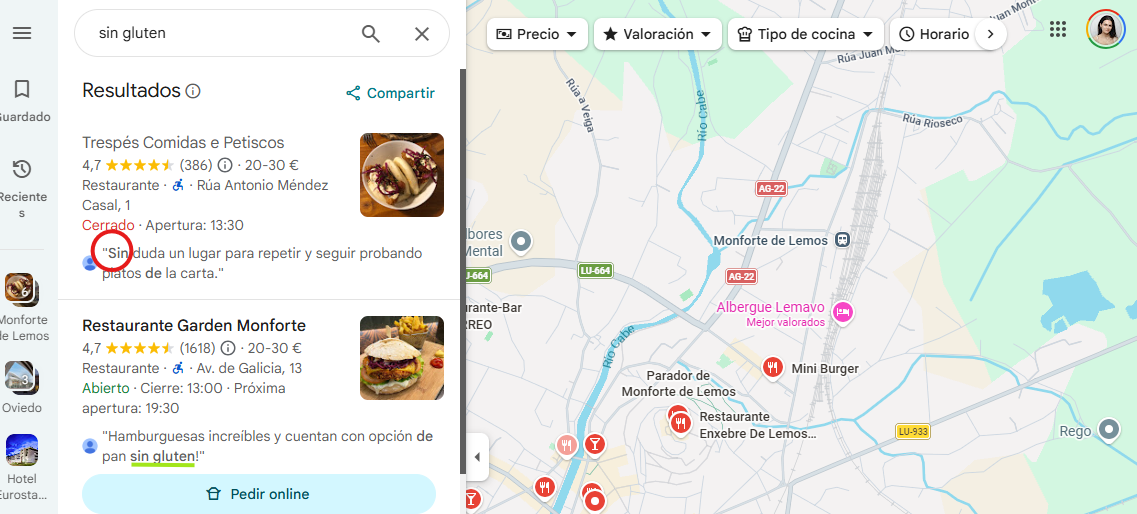
\includegraphics[height=5cm]{images/lugaresPrueba.png}
\end{center}

\vspace{4cm}
\subsection{Definición de la Propuesta}

La propuesta del proyecto se basa en intentar \textbf{satisfacer una necesidad que se puede cubrir creando una aplicación para móvil} donde los usuarios puedan buscar establecimientos cerca de su ubicación o en otros lugares que dispongan de menú alternativo sin gluten.

Para confirmar la veracidad de los establecimientos, otros usuarios que padecen de la misma enfermedad comentarán su experiencia y le dará más credibilidad a los lugares a los que otros usuarios no hayan ido.

\vspace{0.5cm}
\subsection{Objetivos del Proyecto}
\subsubsection{Objetivo General}
El objetivo principal del proyecto es \textbf{diseñar y desarrollar una solución al problema plantado anteriormente mediante una aplicación móvil que garantice a los usuarios que están buscando sitios sin gluten} recomendados por otras personas que también son celiacas o intolerantes. 

\subsubsection{Objetivos Específicos}

\begin{itemize}
    \item Conseguir que ya no sea necesario ese círculo cercano para obtener información y haya un inventario digital muy completo actualizando los locales que vayan apareciendo sin gluten. 
    \item Conseguir esa fiabilidad mediante las experiencias reales de los usuarios con las valoraciones y comentarios. 
    \item Intentar facilitar la búsqueda de los establecimientos en tiempo real mediante el uso de mapas interactivos.
    \item Desarrollar una única base con React Native y Expo para asegurar la compatibilidad en Android/iOS.
    \item Diseñar una arquitectura de base de datos no relacional en MongoDB que vaya a almacenar información escalable y flexible para futuras mejoras.
    \item Implementar el SDK de Google Maps para la visualización y filtrado por ubicación del usuario.
    \item Diseñar una interfaz intuitiva y accesible en la que puedas encontrar un establecimiento en 5 minutos.
\end{itemize}

\vspace{1cm}
\section{Análisis de Requisitos}
\subsection{Requisitos Funcionales}
Los usuarios van a poder realizar las siguientes acciones dependiendo de que quiera hacer:

\textbf{Gestionar el Perfil y Usuario}
\begin{itemize}
    \item \textbf{RF1 - Inicio de Sesión y Registo:} el usuario tiene que poder crear una cuenta de forma intuitiva y poder iniciar sesión con la misma enseñado validaciones para que el usuario pueda ver si tiene un error o está todo correcto.
    \item \textbf{RF2 - Gestionar su Perfil:} el usuario tiene que pode reditar sus datos personales si le interesa o cerrar cesión.
\end{itemize}

\vspace{0.5cm}
\textbf{Buscar Establecimientos y Localización}
\begin{itemize}
    \item \textbf{RF3 - Localización en tiempo real:} la aplicación tiene que cargar la ubicación del usuario a través del GPS del móvil.
    \item \textbf{RF4 - Ver en Mapa:} poder ver los establecimientos cercanos sin gluten a través de Google Maps.
    \item \textbf{RF5 - Buscador con Filtros:} el buscador tiene que poder filtar por nombre del establecimiento, lugar y valoraciones.
\end{itemize}

\textbf{Información Adicional de los Establecimientos}
\begin{itemize}
    \item \textbf{RF6 - Fichas de establecimientos:} El usuario al darle a un establecimiento puede ver la Información detallada del mismo, con sus fotos, dirección, teléfono y comentarios de otros usuarios.
    \item \textbf{RF7 - Creación de Reseñas y Valoraciones:} los usuarios pueden valorar los establecimientos a través de una puntuación de 1 a 5 estrellas y añadir un comentario.
\end{itemize}

\textbf{Administración de lugares}

\textbf{RF8 - Creación de los establecimientos:} un administrador tiene que poder añadir neuvos establecimientos a la base de datos de MOngoDB.

\vspace{0.5cm}
\subsection{Requisitos No Funcionales}
Estos requisitos son los que definen la calidad del sitema:

\textbf{RNF1 - Seguridad:} las contraseñas en la base de datos deberían estar encriptadas.

\textbf{RNF2 - Usabilidad:} la interfaz tiene que ser intuitiva para que el usuario se sienta cómodo al usar la aplicación siguiendo unas bases de diseño funcional.

\textbf{RNF3 - Rendimiento:} las consultas que realicen los usuarios a la API Express no puede superar un tiempo de respuesta considerado largo.

\vspace{0.5cm}
\subsection{Historias de Usuario}

\textbf{Bloque Administrador}

\begin{table}[h]
    \centering
    \begin{tabular}{|p{1.5cm}|p{5cm}|p{8cm}|}
    \hline
    ID & Historias de Uso & Criterios de Aceptación \\ \hline
    HU-06 & Como administrador tengo que borrar un establecimiento porque ya no posee una alternativa sin gluten. & 1. Seleccionar el local. 2. Borrar a través del botón y doble confirmación.\\ \hline
    HU-07 & Como administrador, quiero validar un nuevo establecimiento para asegurar que la información de la app es verídica.  & 1. El admin recibe una notificación de nuevo local. 2. Puede editar los datos del local antes de subir. 3. Al confirmar, el local aparece para todos. \\ \hline
    HU-08 & Como administrador tengo que borrar los comentarios innapropiados. & 1. Seleccionar el local. 2. Seleccionar la reseña innapropiada. 3. Borrar a través del botón y la doble confirmación. \\ \hline
    \end{tabular}
\end{table}

\vspace{3cm}
\textbf{Bloque Búsqueda}
\begin{table}[h]
    \centering
    \begin{tabular}{|p{1.5cm}|p{5cm}|p{8cm}|}
    \hline
    ID & Historias de Uso & Criterios de Aceptación \\ \hline
    HU-03 & Como usuario celíaco, quiero ver un mapa con locales cercanos para encontrar dónde comer sin desplazarme mucho. & 1. El mapa muestra la ubicación actual del usuario. 2. Se ven marcadores de los locales "sin gluten". 3. Al pulsar un marcador, se ve el nombre del local.\\ \hline
    HU-04 & Como usuario quiero filtrar un establecimiento por el nombre. & 1. En el buscador del mapa, escribir el nombre del local. 2. Darle al botón de buscar. 3. Marcadores de los sitios con ese mismo nombre. \\ \hline
    HU-05 & Como usuario quiero ver una ficha detallada de un local para contactar con él.  & 1. Buscar un local. 2. Seleccionarlo y se muestra la ficha del local. \\ \hline
    \end{tabular}
\end{table}

\textbf{Bloque Usuarios}
\begin{table}[h]
    \centering
    \begin{tabular}{|p{1.5cm}|p{5cm}|p{8cm}|}
    \hline
    ID & Historias de Uso & Criterios de Aceptación \\ \hline
    HU-01 & Como usuario necesito crear una cuenta para acceder a la aplicación. & 1. Usuario rellena formulario de registro. 2. Crear la cuenta. 3. Ahora puede iniciar sesión.\\ \hline
    HU-02 & Como usuario tengo que poder entrar con la cuenta que he creado.  & 1. El usuario rellena le formulario con el correo y contraseña. 2. Accedea la app si las credenciales son correctas. \\ \hline
    \end{tabular}
\end{table}

\textbf{Bloque Reseñas}
\begin{table}[h]
    \centering
    \begin{tabular}{|p{1.5cm}|p{5cm}|p{8cm}|}
    \hline
    ID & Historias de Uso & Criterios de Aceptación \\ \hline
    HU-09 & Como usuario quiero ver las reseñas de un local en específico. & 1. Se busca un local y se selecciona. 2. Se obtiene la información del local más las reseñas publicadas.\\ \hline
    HU-10 & Como usuario quiero subir una reseña de un local en el que estuve.  & 1. Se busca un local y se selecciona. 2. Dar al botón de añadir reseña. 3. Rellenar formulario y enviar. \\ \hline
    \end{tabular}
\end{table}

\vspace{0.5cm}
\subsection{Diagrama de Casos de Uso}

El diagrama representa las interacciones principales del Usuario con la aplicación y el Administrador gestionado la aplicación. Por un lado, hay Actores en este caso el Usuario y el Administrador están representando los "stickman" a la izquierda. A continueación se describen las relaciones clave para explicar el flujo y las dependencias de las acciones. Las acciones que necesitan realizar necesitan iniciar sesión con una cuenta. 

El \textbf{Usuario} puede de primeras registrarse si no lo está y luego iniciar sesión o directamente iniciar sesión. Tras tener la cuenta iniciada puede:
\begin{itemize}
    \item \textbf{Buscar un local en el mapa} mediante un buscador que filtra según lo escrito y marca en el mapa el local.
    \item \textbf{Consultar ficha local} luego de la búsqueda anterior o a través del menú de locales seleccionas el local y entras en su informaciónd detallada que permite añadir a la lista de favoritos.
    \item \textbf{Crear Reseñas y consultarlas} dentro de la ficha del local se ve la lista de las reseñas y mediante un formulario se puede añadir un comentario junto a una puntuación. Que luego se pueden ver en el apartado del menú principal de la aplicación.
    \item \textbf{Añadir a Favoritos y consultarlos} en al ficha puedes añadir ese local a tu lista de favoritos y verlos en un apartado del menú principal.
\end{itemize}

El \textbf{Administrador} luego de iniciar sesión con su usuario dado puede realizar las siguientes operaciones: 
\begin{itemize}
    \item \textbf{Añadir/Editar/Borrar un local} mediante unos formularios el administrador puede realizar esas acciones según lo que interese y guardar los cambios en ese momento.
    \item \textbf{Borrar Comentarios} que se consideren innapropiados o fuera de lugar a través de un botón y boble confirmación.
\end{itemize}

\vspace{0.5cm}
\begin{center}
    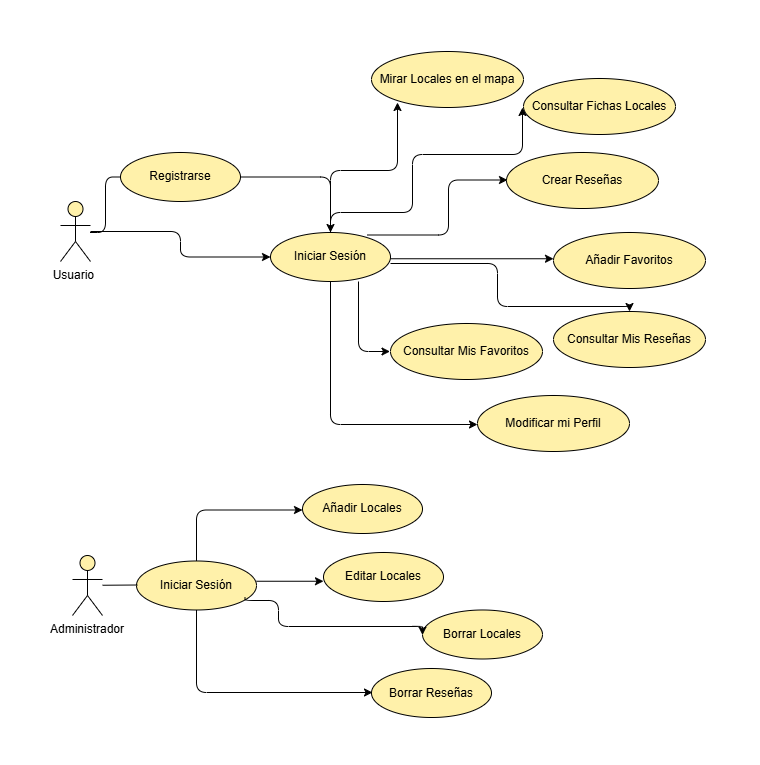
\includegraphics[height=16cm]{images/diagramaCaso.png}
\end{center}

\vspace{0.5cm}
\subsection{Esquema Entidad - Relación}

Se ha elaborado el modelo Entidad-Relación  para reprensetar la estructura lógica de los datos de la aplicación. En el modelo se identifican las entidades principales \textbf{(Usuario, Establecimiento, Reseña y Administración)} y los atributos.

Este esquema sirve de base para la posterior implementación de las colecciones en el sistema de base de datos NoSQL seleccionado (MongoDB).

\begin{center}
    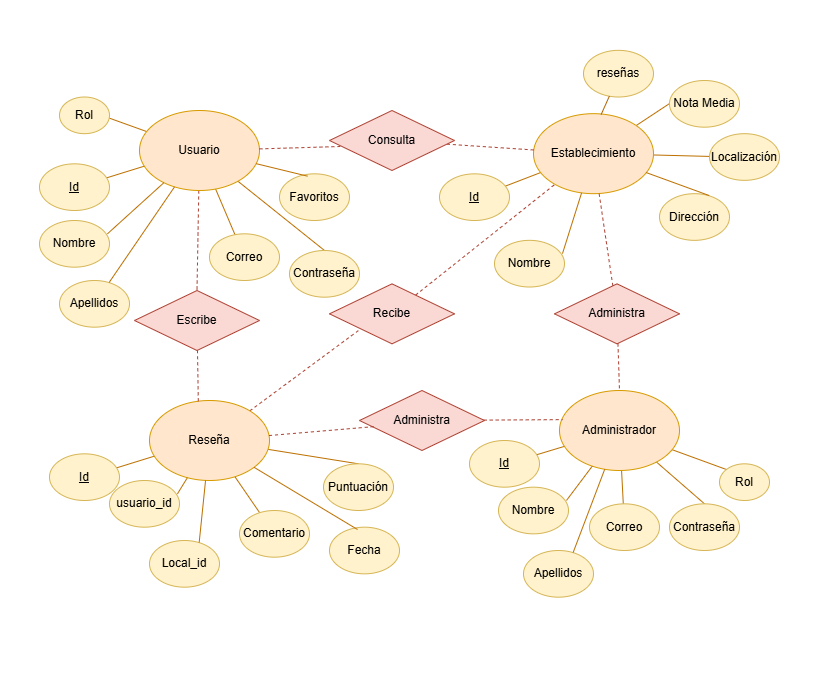
\includegraphics[height=12cm]{images/DiagramaEntidadRelacion.drawio.png}
\end{center}

\vspace{0.5cm}
\subsection{Diagrama de Clases}

Para organizar la información de la aplicación, se ha diseñado un diagrama de clases que muestra cómo se relacionan los datos principales. Aunque usamos \textbf{MongoDB}, este esquema nos ayuda a estructurar el código en el servidor.

\textbf{Definición de las clases}
\begin{itemize}
    \item \textbf{Usuario}: guarda los datos de las personas que usan la app (atributos) en la que tiene una lista de \textbf{favoritos} que permite al usuario guardar sus locales preferidos en una lista y verlos todos juntos.
    \item \textbf{Establecimiento}: tiene una ficha por cada restaurante que se añada y se guarda la \textbf{Localización exacta} usuando el tipo "Point" para que aparezcan en el mapa, además de la nota media de los usuarios que publiquen una reseña sobre ese establecimiento.
    \item \textbf{Reseña}: es el comentario que escribe un usuario sobre un local viculando a la persona con el local obteniendo su puntuación y fecha del comentario.
    \item \textbf{Administrador}: es el usuario especial que tiene permitido \textbf{añadir, editar o borrar locales o borrar comentarios innapropiados} para ir manteniendo la aplicación actualizada.
\end{itemize}

\textbf{Conexión entre las clases}
\begin{itemize}
    \item \textbf{Un usuario puede escribir muchas reseñas}, pero cada reseña es escrita por un único usuario solo.
    \item \textbf{Un local puede recibir muchos comentarios}, pero cada reseña va a un local en específico.
    \item \textbf{Los favoritos} es una relación libre donde muchos usuarios pueden guardar muchos locales diferentes para verlos a parte.
\end{itemize}

\vspace{0.5cm}
\begin{center}
    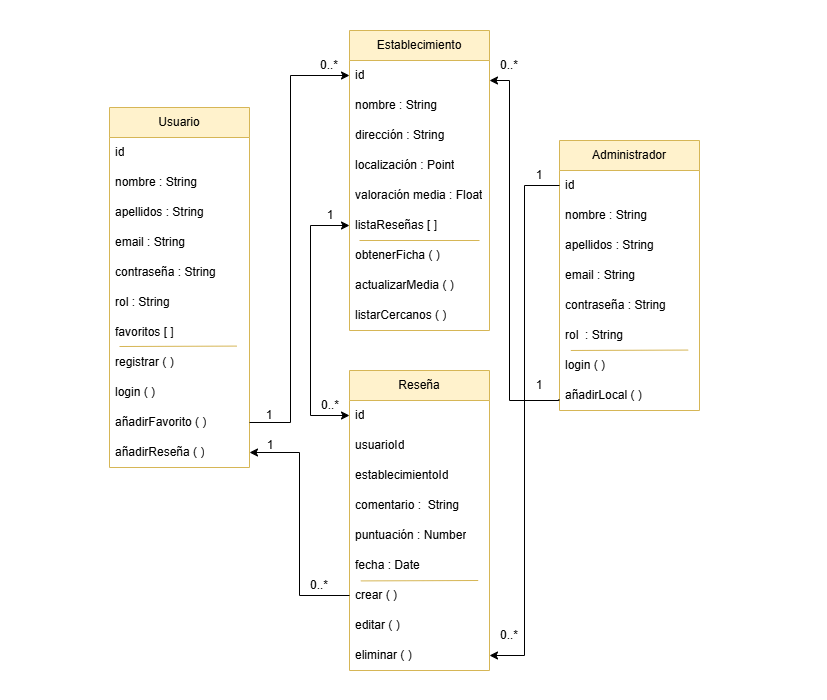
\includegraphics[height=12cm]{images/DiagramaClases.drawio.png}
\end{center}

Por lo que este diseño permite que la aplicación sea rápida y que los datos estén siempre bien organizados ayudando a que las personas puedan buscar un sitio sin gluten cerca de su ubicación de forma eficiente.

\section{Tecnologías Utilizadas}

Para la realización del proyecto en este apartado se definen las herramientas y lenguajes que se van a necesitar dividiendo en 3 capas: Frontend (Móvil), Backend (API) y Persistencia (Base de Datos). 

\subsection{Frontend : Móvil}
Para el desarrollo del Frontend se va a utilizar React Native + Expo. 
\begin{itemize}
    \item \textbf{React Native} va a permitir crear la aplicación móvil usando JavaScript y React. Que a diferencia de las aplicaciones web, React Native renderiza componentes nativos por lo que ofrece una experiencia de usuario más fluida. \cite{2}
    \item \textbf{Expo}  se compone por un conjunto de herramientas y servicios construidos alrededor de React Native. Esto facilita el acceso al GPS, la cámara y el despliegue. Expo Go o Android Studio para ir viendo en tiempo real los cambios que se van realizando y para los testeos. \cite{3}
\end{itemize}

\subsection{Backend}

Para el desarrollo de Backend se va a implementar Node.js + Express. Esta combinación va a permiter crear una API REST eficiente y robusta.\cite{4} Se escogieron porque así se unifica el lenguaje usando solamente JAvaScript tanto en el Frontend como en el Backend por lo que es más fácil intercambiar modelo de datos mediante JSON.
\subsection{Base de Datos}
Parar su desarrollo se utilizará un modelo de base de datos no relacional por si en algún comento se quiere añadir más atributos, se puedan añadir fácilmente, en este caso se usará MongoDB.

Por lo que en resumen el stack tecnológico será el siguente:
\begin{itemize}
    \item Frontend: React Native + Expo
    \item Backend: Node.js + Express
    \item Base de Datos: MongoDB
\end{itemize}

\begin{center}
    
\includegraphics[height=2cm]{images/herramientas0.png}
\end{center}

\vspace{1cm}
\subsection{Herramientas Auxiliares}
Para dar soporte al desarrollo y asegurar la calidad del proyecto se han utilizado otras herramientas implementadas en otros proyectos:
\begin{enumerate}
    \item \textbf{Git y GitHub} para control de versiones, que permite tener un historial de cambios, trabajar en diferentes ramas y asegurar de tener el código en la nube como respaldo.
    \item \textbf{Postman} para pruebas de la API antes de conectar con React Native para probar los endpoints de la API Express, verificando si las rutas devuelven el JSON correcto.
    \item \textbf{MongoDB Atlas y Compass}:
    \begin{itemize}
        \item MongoDB Atlas es un servicio en la nube donde se aloja la base de datos real y que permite que la app sea accesible desde cualquier lugar no solo a nivel local.
        \item MongoDB Compass es una app de escritorio que permite visualizar los documentos y ver consultas de forma visual.
    \end{itemize}
    \item \textbf{Visual Studio Code} es el IDE que principal que tiene extensiones para JavaScript y React Native que centraliza todo el desarrollo de la aplicación.
    \item \textbf{Figma} es una herramienta de diseño de interfaces que será la base del diseño del prototipado de la aplicación, definiendo una línea gráfica con colores, botones, iconos además de la identidad de la aplicación.
    \item \textbf{Bcrypt} es una librería de cifrado y "haseo" de contraseñas, que al usuario registrarse la librería convierte la contraseña en una cadena de caracteres aleatorios. Por lo que no puede saber las contraseñas ni siendo administrador.
    \item \textbf{Dotenv} carga variables de configuración desde el archivo externo .env donde se guardará en este proyecto la URL de la base de datos MongoDB Atlas, las claves o la clave de los tokens JWT.
\end{enumerate}

\begin{center}
    
\includegraphics[height=1.8cm]{images/herramientas.png}
\end{center}

\section{Diseño del Sistema}
\subsection{Arquitectura de la App Cliente-Servidor}

En la arquitectura cliente-servidor participan dos componentes: por una parte el cliente que utiliza unos servicios y por otra parte el servidor que ofrece esos servicios. Entre ellos se tiene que establecer una comunicación mediante principalmente internet.

El\textbf{ rol Cliente} va a ser la parte de la aplicación que inicia las diversas peticiones de servicios al servidor usando la red como medio de comunicación. En el cliente se encuentra toda la funcionalidad que permite al usuario interactuar mediante una interfaz que refleje la idea de la identidad de la aplicación y que sea lo más funcional posible.

El\textbf{ rol Servidor} es el componente que se encarga de recibir y responder a las peticiones solicitadas desde la aplicación cliente (frontend). En este caso el servidor está desarrollado en Node.js y Express, el que actua de intermediario con la base de datos. Su función principal es gestionar la comunicación de manera segura con la base de datos MongoDB Altas y devolver las respuestas correspondientes en formado JSON. Al estar de forma externa del cliente, hace que los datos sensibles y el proceso pesado no afecten al rendimiento del móvil del usuario.

\subsection{Diseño de la Base de Datos}

Teniendo en cuenta que la aplicación requiere tratar con geolocalización de locales y de reseñas se optó por un diseño de base de datos no relacional utilizando MongoDB. Ya que en comparación a los modelos relacionales, la estructura se organiza en colecciones flexibles de documentos JSON por lo que optimiza las consultas.

El diseño se compone de tres colecciones principales que están conectadas entre sí de manera lógica:
\begin{itemize}
    \item \textbf{Usuarios}: Almacena la información de los usuarios y los registros de los mismos, incluyendo los campos siguientes: (id, nombre, apellidos, foto de perfil, correo, contraseña y lista de locales favoritos).
    \item \textbf{Locales}: Cuenta con todos los locales aptos para celíacos e intolerantes con los siguientes datos: (id, nombre, foto del local, tipo(restaurante, supermercado y cafetería), direccion, ubicacion (latitud y longitud), web y nota media del local).
    \item \textbf{Reseñas}: Viculadas a un usuario y a un establecimiento escogido por el usuario en el que consta de los siguientes datos: (id usuario, id local, nombre local, comentario, nota (1 al 5)).
\end{itemize}

\subsection{Diseño de la API REST}
Para la comunicación entre la aplicación móvil (cliente) y el servidor se realizar mediante el diseño de una interfaz de programación de aplicaciones basada en la arquitectura API REST. \cite{5} El paso de datos se realizar bajo el protocolo HTTP/HTTPS utilizando verbos estandarizados para definir las operaciones:
\begin{itemize}
    \item \textbf{POST /api/login}: Para acceder a la aplicación y tras crear un usuario propio a través del registro, se introduce el correo y la contraseña creada y si esos datos son validos al compararlos con los datos de la base de datos se accede a la aplicación.
    \item \textbf{POST /api/registro}: El usuario a través de un formulario, rellena con sus datos y se guardan de forma segura creando un nuevo usuario que podrá iniciar sesión luego de que todos los datos esén bien validados.
    \item \textbf{POST /api/locales/crear}: A través de un formulario que rellena el administrador, se cogen esos datos y se va a poder crear un nuevo local que se añadirá a la lista de los demás locales.
    \item \textbf{POST /api/locales/resena}: Un usuario a través de un pequeño formulario que encuentra dentro de las fichas individuales de los locales, esos datos se recogen para crear una nueva reseña que se añade a la lista de comentarios que tiene ese establecimiento.
    \item \textbf{POST /api/locales/favorito}: Dentro de la ficha de un local hay un botón de un corazón donde el usuario al pinchar sobre él. Esta ruta coge el id del usuario y lo añade a la lista de favoritos de ese local. Luego el usuario tiene su propia lista con todos los comentarios que ha creado.
    \item \textbf{GET /api/locales/:id}: Para enseñar una ficha detallada de un local se necesita recuperar un id del local seleccionado para poder mostrar los datos que contiene.
    \item \textbf{GET /api/locales}: Obtener todos los locales para luego enseñarlos al usuario según la cercanía, el tipo de local o el nombre. 
    \item \textbf{GET /api/locales/buscar}: Para encontrar un local, el usuario tiene que buscarlo por el nombre del local o por palabras clave que busca por cercanía para luego enseñarlo en la lista del buscador de google maps. 
    \item \textbf{GET /api/locales/favoritos/:usuarioId}: Para enseñar las reseñas de un local se necesita obtener el id de los usuarios para enseñar tanto el comentario como a la nota.
    \item \textbf{POST USUARIOS AÑADEN RESEÑAS}: EL usuario a través de un formulario que encuentra dentro de cada local en el que tiene que añadir un comentario y del 0 al 5 las estrellas que considere, esos datos se guardan y se pasan a la API que los almacena como nueva reseña.
    \item \textbf{POST /api/locales/crear}: Los datos que rellena el admin a través del formulario se recoge y se envia a la API que los junta para crear un nuevo local que se añadir al resto ya creados.
    \item \textbf{PUT USUARIO EDITA RESEÑA}: El usuario va a tener un formulario por cada reseña que tenga que le permita modificar su reseña, esos datos se guardan y la api los sustituye por los anteriores datos.
    \item \textbf{PUT USUARIO EDITA DATOS PERFIL}: Por cada elemento del perfil del usuario va a poder editar, esos datos se guardan y se sobrescriben sobre los originales de la base de datos.
    \item \textbf{PUT /api/locales/actualizar/:id}: El admin al escoger un local se guarda el id y nos enseña el mismo formulario que para crear local pero con los datos actuales del establecimiento, el admin los puede modificar y actualizar, los nuevos datos de mandan a la api y se sobrescriben sobre los datos anteriores.
    \item \textbf{DELETE ADMIN BORRA UN LOCAL}: El admin escoge un local, se guarda el id y tiene un botón que le permite eliminar ese local mediante un modal para una doble confirmación, esa petición de borrado se manda a la api y ese local queda eliminado de la base de datos.
\end{itemize}

\subsubsection{Seguridad (JWT, validación Zod y bcrypt)}

La arquitectura de la API REST se ha diseñado de manera híbrida en la que los endpoints orientados a la consulta de los locales e información general son públicos para optimizar el rendimiento, mientras que los endpoints que manejan los datos sensibles del usuario se encuentran protegidos mediante Tokens JWT. Lo que garantiza al usuario poder acceder a sus propios datos de manera segura sin riesgos a tener filtaciones de ids.

En Kivaa el ciclo de vida del token es el siguiente: 
\begin{enumerate}
    \item \textbf{Inicio de Sesión y almacenamiento}: el usuario al introducir su correo y contraseña en la pantalla de Login envía estos datos a la API al verificar que son correctas se genera un Token de acceso (que es una clave única y temporal) y se devuelve a la aplicación. El usuario para que no tenga que introducir la contraseña cada vez que abre la aplicación el token tiene que estar guardado en el móvil. Por lo que se ha integrado la librería "expo-secure-store" que permite almacenar el token en una zona restringida del móvil, que es portegida por el propio sistema operativo.
    \item \textbf{Comunicación Protegida de la APP con la API}: al tener guardado el token en el dispositivo cada vez que se realice una petición que contenga datos del usuario la aplicación necesita identificarse ante la API. Para no enviar el envío en cada pantalla del Token, con la librería "Axios" 
    \item \textbf{Cierre de Sesión}: El token generado ya no existe cuando el usuario decide cerrar sesión y envía al usuario de nuevo a la pantalla de inicio de sesión. \cite{6}
\end{enumerate}

\vspace{0.5cm}

\begin{lstlisting}[style=javascript, caption={Generar Token al iniciar sesión el usuario.}]

    app.post("/api/login", async (req, res) => {
    try {
        ...
        // JWT,generar Token
        const token = jwt.sign(
            { id: usuario._id,nombre: usuario.nombre, role: usuario.role, apellidos: usuario.apellidos, clave: usuario.clave},
            JWT_SECRET,
            { expiresIn: '2h' }
        );

        res.json({
            token,
            usuario: {
                id: usuario._id,
                nombre: usuario.nombre,
                apellidos: usuario.apellidos,
                email: usuario.email,
                role: usuario.role,
                clave: usuario.clave
            }
        });
    } catch(error) {
        res.status(500).json({ message: "Error del servidor" });
    }
});
\end{lstlisting}

El token generado se va a tener que verificar a través de una función que se ejecuta antes de que la petición llegue a la ruta. Si el token no existe o es inválido, corta la comunicación y devuelde un error. 

\vspace{0.8cm}

\begin{lstlisting}[style=javascript, caption={Middleware para proteger rutas con jwt}]

const verificarToken = (req, res, next) =>{
    //Extrae la cabecera de los headers enviados
    const authCabecera = req.headers["authorization"];
    //Formato estandar "Bearer <TOKEN>" 
    const token = authCabecera && authCabecera.split(' ')[1];
    //Si no hay token, devuelve error
    if (!token) {
        return res.status(401).json({ message: "Acceso denegado. No se proporciono un token." });
    }
    try{
        //El token tiene que ser veridico y que no haya caducado
        const verificado = jwt.verify(token, JWT_SECRET);
        // Meten los datos decodificados del usuario en el objeto "req"
        req.usuario = verificado;
        //Y ahora se va a la ruta 
        next();
    }
    catch(error){
        return res.status(403).json({ message: "Token invalido o caducado." });
    }
}
\end{lstlisting}

Para proteger a los endpoints, por ejemplo el del filtrado de los locales favoritos de un usuario, se inyecta el middleware después de la ruta. Gracias a "req.usuario" se sabe que usuario está pidiendo los datos: 

\vspace{0.5cm}

\begin{lstlisting}[style=javascript, caption={Ejemplo de ruta con middleware}]

app.get("/api/locales/favoritos", verificarToken, async (req, res) => {
    // Al pasar el middleware, req.usuario ya existe y contiene el ID extraido de forma segura
    const usuarioId = req.usuario.id;
    const listaFavoritos = await Locales.find({ favoritos: usuarioId });
    return res.json(listaFavoritos);
});

\end{lstlisting}

En el front, se inicia sesión, el token se almacena en el almacenamiento persistente del dispositivo mediante "AsyncStorage". Cuando el usuario navega a una pantalla en la que la petición tenga que ver con información del usuario (como ver los locales favoritos), se extrae el token del almacenamiento local y lo adjunta en los Headers de la petición HTTP utilizando Axios.

\vspace{0.5cm}

\begin{lstlisting}[style=javascript, caption={Funcionamiento en el Frontend}]

useFocusEffect(
  useCallback(()=>{
    const datosUsuario = async () => {
      try {
        const nombre = await AsyncStorage.getItem("nombreUsuario");
        const usuarioId = await AsyncStorage.getItem("idUsuario");
        const fotoGuardada = await AsyncStorage.getItem("fotoUsuario");
        // Se recupera el token guardado fisicamente en el dispositivo
        const token = await AsyncStorage.getItem("token");
        if(nombre){
          setNombreUsuario(nombre);
        }
        // Si el token existe, configuramos la peticion HTTP
        if(token){
          const resultado = await axios.get(`http://10.0.2.2:3000/api/locales/favoritos`,{
            // Cumplimos con el estandar pasando el token en las cabeceras de autorizacion
            headers:{
              Authorization: `Bearer ${token}`
            }
          });
          // Procesamos los datos devueltos de forma segura por el servidor
          const idsFavoritos = resultado.data.map((fav: any) => fav._id);
          setFavoritos(idsFavoritos);
        }
        if (fotoGuardada) {
          setFotoUsuario(fotoGuardada);
        } else {
          setFotoUsuario(null);
        }
      }
      catch(error){
        console.error("Error al cargar los datos", error);
      }
    };
    datosUsuario();
  }, [])
)

\end{lstlisting}

Para seguir mejorando la seguridad de los datos en la API se implementa un sistema de validación de datos y del cliente (Zod) y el encriptado de las contraseñas de los usuarios (Bcrypt).

La \textbf{librería Zod} se encarga en tiempo real de que los campos cumplan los requisitos (por ejemplo: que el correo tenga el formato correo con @, o que los nombres y apellidos tengan una longitud mínima). Si los campos no cumplen con los requisitos la app bloquea la petición HTTP y enseña un mensaje de error al usuario en la aplicación. Esto aporta que el cliente sabe que contenido tiene que insertar y cuando se está equivocando, haciendo la experiencia de usuario más fácil. \cite{7}

\vspace{0.5cm}

\begin{lstlisting}[style=javascript, caption={Ejemplo de validación de datos al registrarse un nuevo usuario.}]

    const { z } = require('zod');

    const RegistroSchema = z.object({
        nombre: z.string().min(2,"Nombre demasiado corto"),
        apellidos: z.string().min(2,"Apellidos obligatorios"),
        email: z.string().email("Email invalido"),
        clave: z.string().min(6, "La clave debe tener al menos 6 caracteres"),
        clave2: z.string()
    }).refine((data) => data.clave === data.clave2, {
        message: "Las contrasenas no coinciden",
        path: ["clave2"],
    });

\end{lstlisting}

Al tener los datos ya validados y llegan a la API lo importante es mejorar la seguridad de las contraseñas de los usuarios y no guardarlas en texto plano. El backend utiliza el algoritmo de función has \textbf{Bcrypt} para encriptar la contraseña antes de guardarla. Esto aplica un proceso de haseo ubilateral junto con una técnica de "saltin" que añade caracteres aleatorios a la contraseña. Por lo que significa que:

\begin{itemize}
    \item Aunque la base de datos sea atacada de forma externa es imposible descifrar las contraseñas de los usuarios.
    \item Al iniciar sesión, Bcrypt \textbf{no desencripta la contraseña, sino que coge la que introduce el usuario y aplica el mismo algoritmo matemático y la compara con la que está en la base de datos.} \cite{8}
\end{itemize}

\vspace{0.5cm}

\begin{lstlisting}[style=javascript, caption={Hasheo de la contraseña en el registro del usuario.}]

    const bcrypt = require('bcrypt');
    //nivel de seguridad
    const saltRounds = 10;

    //Registrarse con los datos y validando que los datos esten correctos
    app.post("/api/registro", async (req, res) => {
        try {
            // Validar con zod
            const validacion = RegistroSchema.safeParse(req.body);
            if (!validacion.success) {
                const erroresFormateados = validacion.error.format();
                return res.status(400).json({ 
                    message: "Error de validacion",
                    detalles: erroresFormateados 
                });
            }
            const { nombre, apellidos, email, clave } = validacion.data;

            const existeUsuario = await Usuario.findOne({ email });
            if (existeUsuario) {
                return res.status(400).json({ message: "El correo ya esta registrado" });
            }

            //Hashear la contrasena y se guarda en el nuevo usuario todos los datos
            const passwordHash = await bcrypt.hash(clave, saltRounds);
            ...
    });

\end{lstlisting}

\subsection{Creación de la Marca y Prototipado de la Interfaz (UX/UI)}
Antes de la realización del prototipado en Figma se ha diseñado una identidad básica de marca que incluye: un \textbf{logotipo, slogan, isotipo, tipografías, paleta de colores (una primaria y algunos colores secundarios) y elementos gráficos} considerados.

Para el nombre se ha elegido Kivaa porque se busca convertir la búsqueda de lugares sin gluten de una experiencia estresante y limitada a una experiencia agradable y fácil. Es una palabra corta que parece inventada pero viene de la palabra \textbf{finlandesa "kiva" que significa "agradable", "divertido"}.

Aquí una muestra básica del branding para tener la primera toma de contacto con la aplicación teniendo una base de la marca y estilos.

\begin{center}
    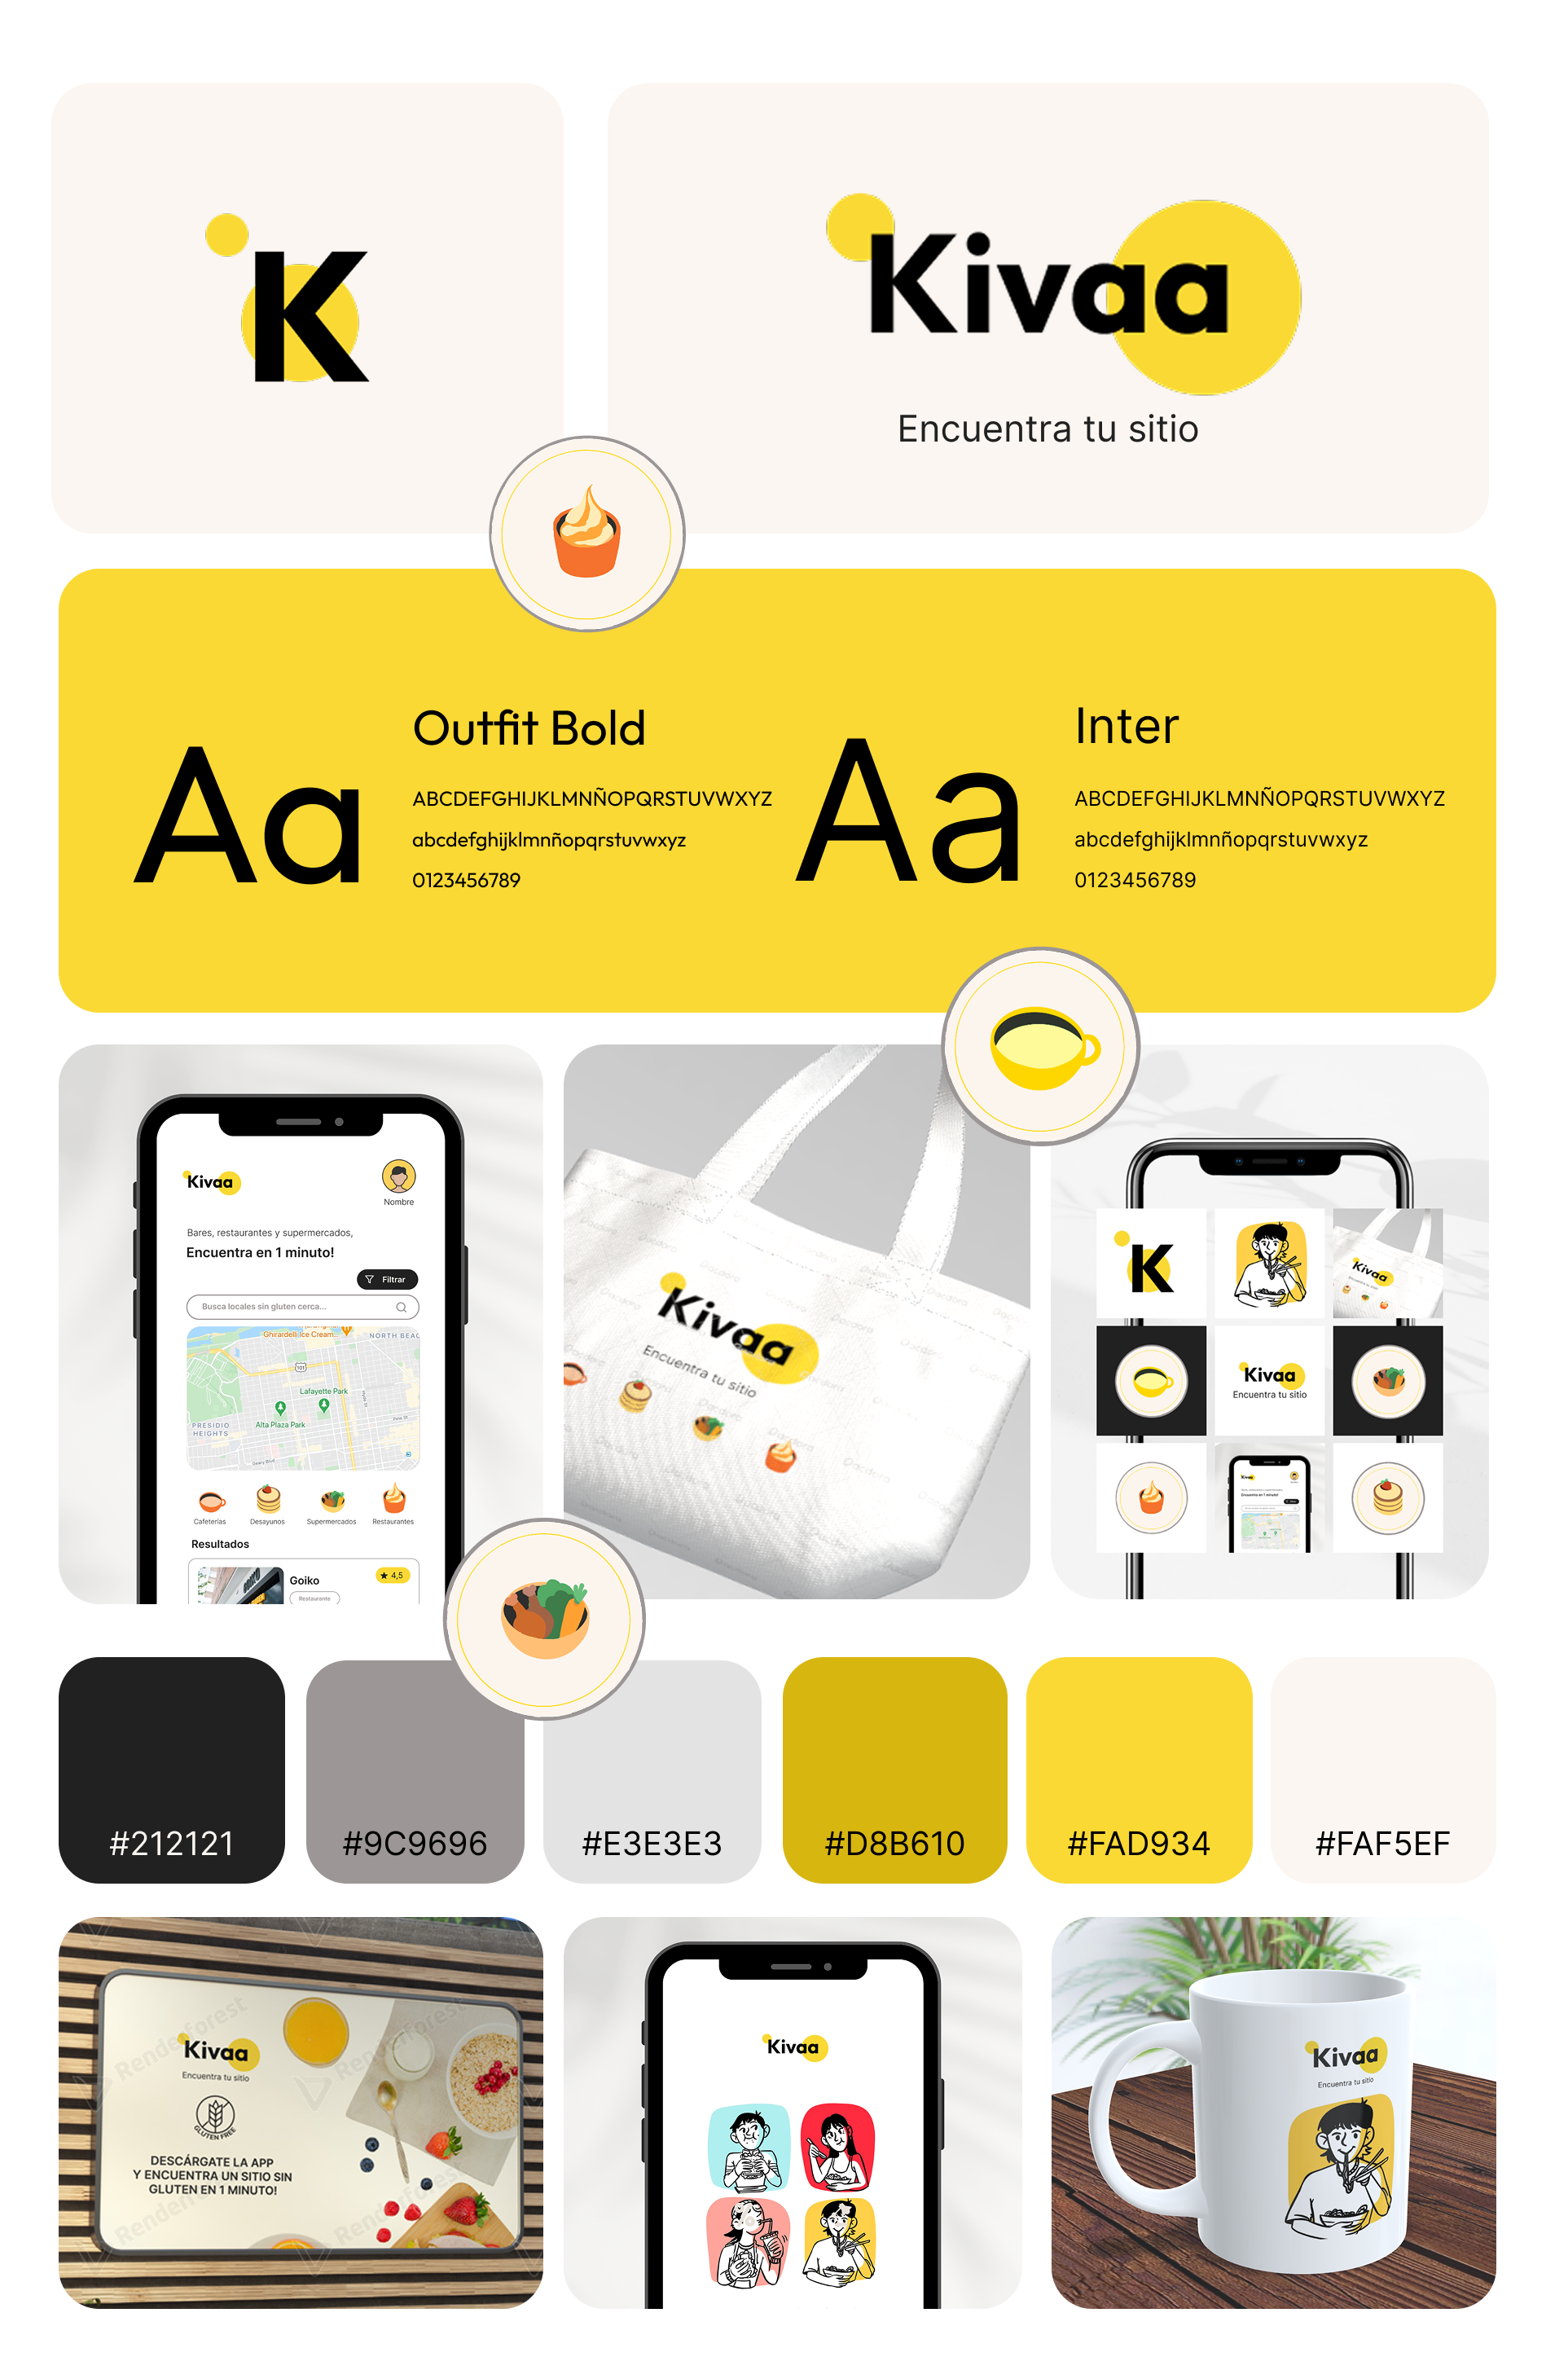
\includegraphics[height=18cm]{images/Branding.png}
\end{center}

Para reflejar esa estética en la aplicación se diseñaron los primeros elementos visuales que tendrá la aplicación en muchas de sus vistas como sería: \textbf{botones, barra de navegación e iconos}. 

\begin{center}
    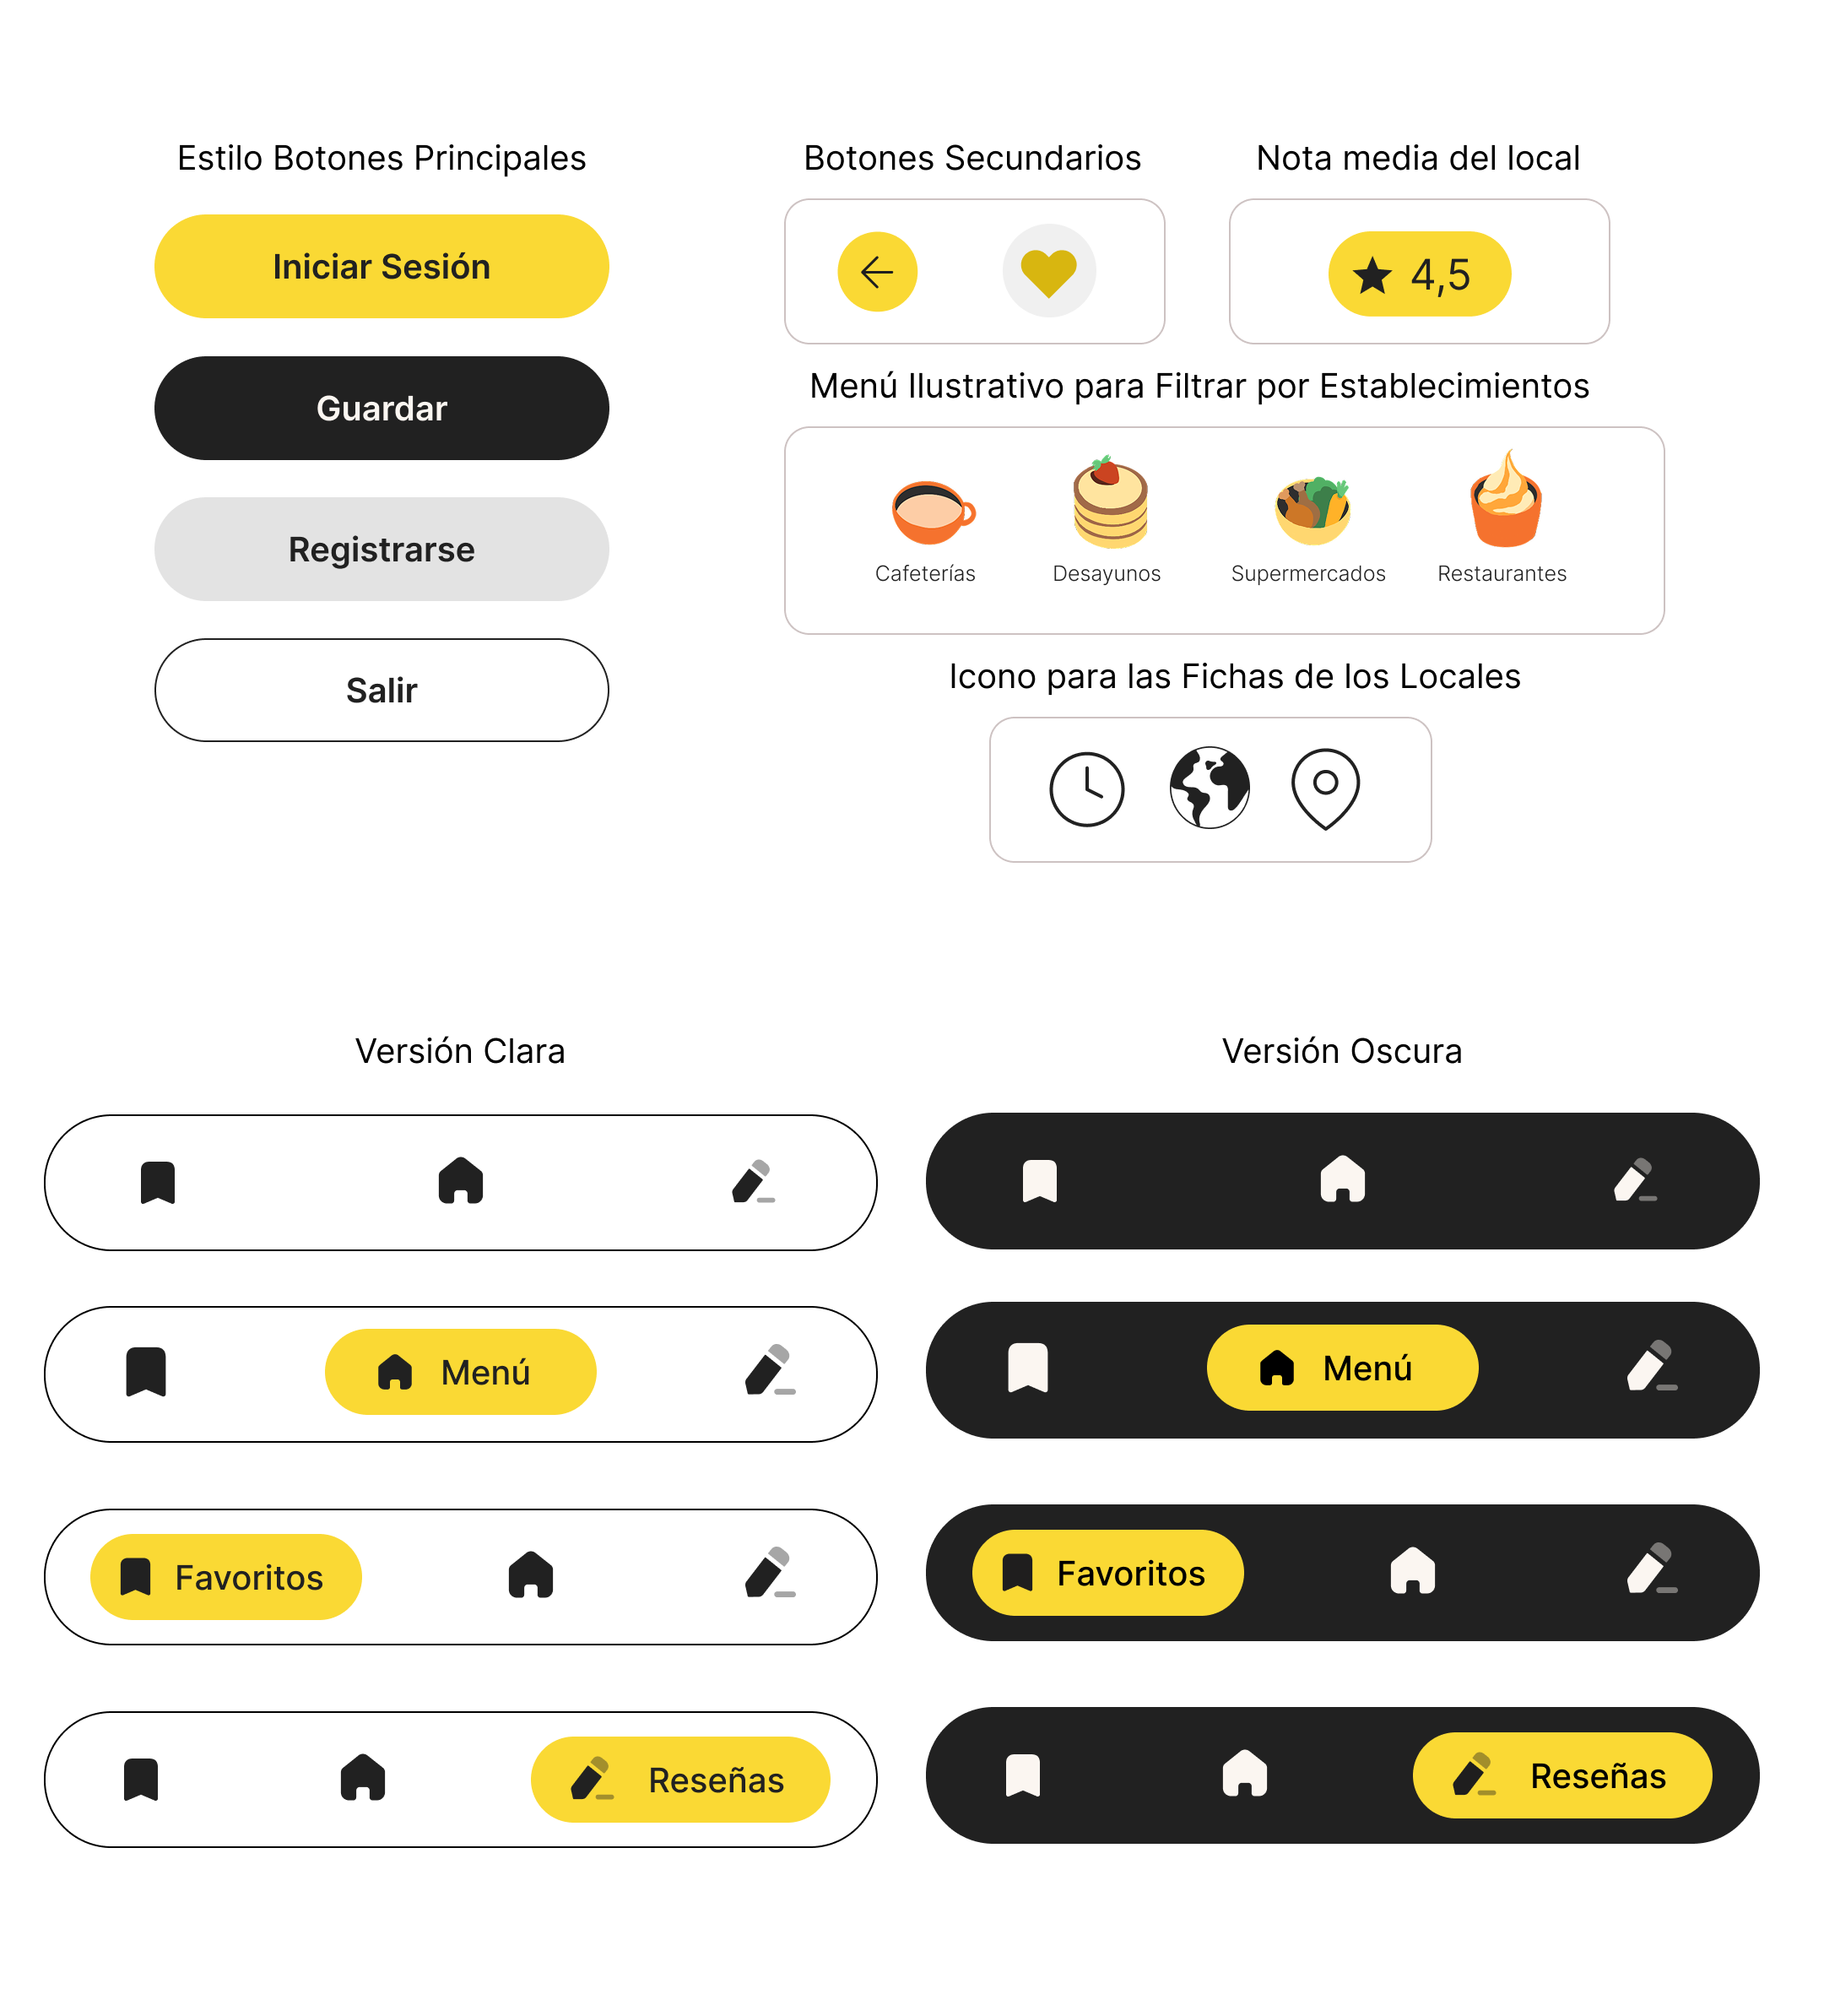
\includegraphics[height=15cm]{images/Iconografia.png}
\end{center}

Al tener la base estética se empezó a desarrollar las vistas principales en Figma. Se realizaron las siguientes propuestas de diseño: \textbf{inicio, inicio de sesión, registrarse, página principal, ficha de local, favoritos, mis reseñas y perfil}. Se intento mantener la misma línea estética en todas las vistas y siempre teniendo en cuenta la mejor usabilidad y facilidad para el usuario. 

A través del enlace a figma \cite{9} se puede probar el prototipado básico de navegación y ver todas las vistas y elementos de la marca creados. Aquí vemos las vistas y que la línea estética sigue en todas ellas. Se diseñaron las vistas del Usuario principalmente porque las vistas del Administrador son la mayoría formularios básicos por lo que al ya tener el de inicio y registro se basaran en ese estilo por lo que se enfocó en detallar el estilo de la versión del usuario.

\begin{center}
    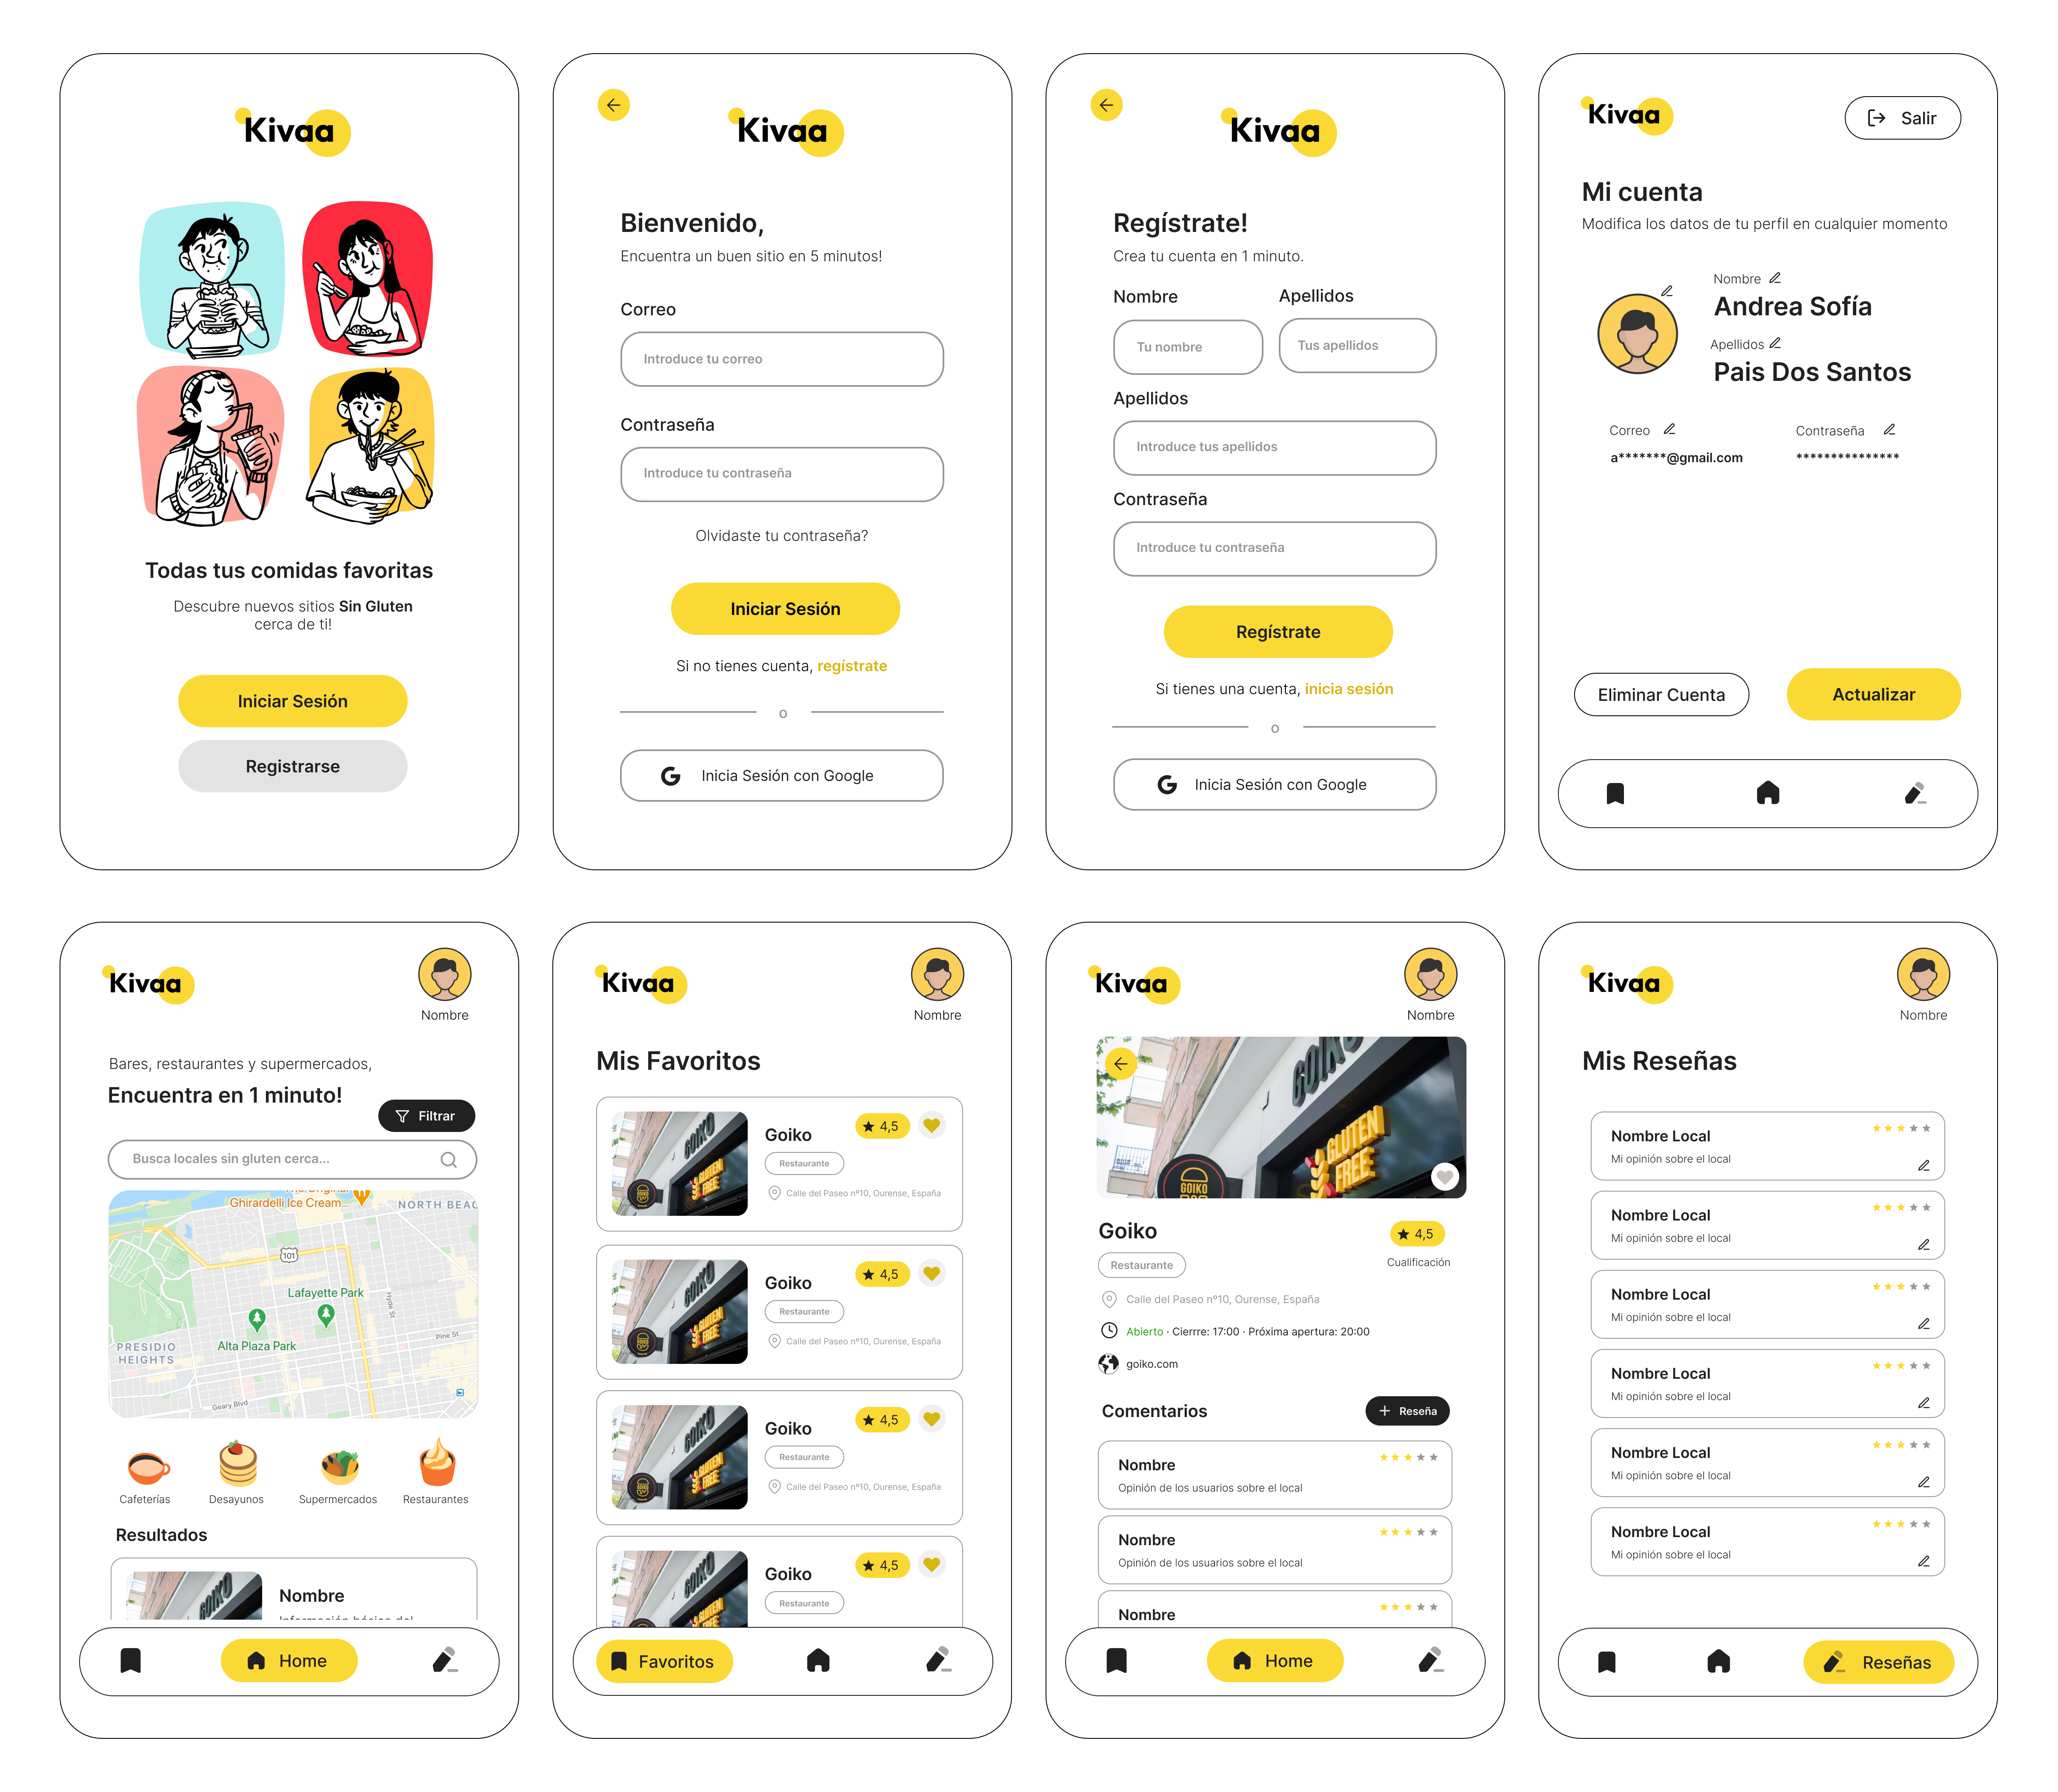
\includegraphics[height=13cm]{images/VistasApp.png}
\end{center}

Ahora a partir del diseño de las vistas se van a implementar en el frontend de la aplicación.  

\section{Desarrollo de la Aplicación Móvil}
Para la creación de la aplicación Kivaa por un lado hay que construir el lado del cliente que es el frontend y luego implementar la conexión a la base de datos a través de la API REST. El desarrollo se ha guiado bajo la reutilización de código, modularidad y optimización a través del framework React Native y las herramientas de despliegue de Expo.

\subsection{Implementación del Frontend}

El Frontend se divide en dos bloques según el rol del usuario: por un lado el cliente y por otro el administrador que gestiona el contenido que tendrá acceso el usuario. Antes de acceder a cada rol hay que \textbf{iniciar sesión} con el corrreo y contraseñas o \textbf{registrarse} con nombre, apellidos, correo y contraseña repetida 2 veces. Al registrar el usuario hay que iniciar sesión otra vez. 

Con el rol de usuario se tendrá acceso:
\begin{itemize}
    \item \textbf{Pantalla Principal} en la que podrá buscar los locales e interactuar con ellos.
    \item \textbf{Pantalla de Locales Favoritos} almacena en una lista los establecimientos el cual el usuario haya interactuado con ellos dándole al icono del corazón.
    \item \textbf{Pantalla Ficha de Local} a través de la pantalla principal o de la de los favoritos se accede a la ficha del local con sus datos detallados en el que se pinche.
    \item \textbf{Pantalla de Reseñas} almacena la lista de comentarios que crea ese usuario de todos los locales y permite editar esos comentarios en cualquier momento.
    \item \textbf{Pantalla de Datos del Usuario} le permite actualizar los datos y cerrar sesión cuando quiera.
\end{itemize}

El lado del administrador cuenta con las siguientes vistas: 

\begin{itemize}
    \item \textbf{Pantalla Principal} tiene unas estádisticas básicas de cuantos locales hay en total y cuantos usuarios hay. Luego cuenta con un menú con varios apartados:
        \subitem \textbf{Crear un Nuevo Local} se crea a través de un formulario que se encuentra en un modal al seleccionar la opción de "Añadir local".
        \subitem \textbf{Editar un Local} se accede a través de la \textbf{Pantalla de Locales} donde primero buscamos el local que queremos modificar. El administrador le da la icono de editar y le abre el mismo modal que el de crear local pero con los datos ya introducidos para cambiarlos y actualizarlos si se necesita.
        \subitem \textbf{Borrar un Local} se accede también a través de la \textbf{Pantalla de Locales} donde se escoge el local y al darle el icono de borrar, tiene que volver a confirmar para eliminarlo.
        \subitem \textbf{Borrar Reseñas}  tiene que navegar a la \textbf{Pantalla de Locales} seleccionar el local y dentro la ficha del local va a ver todos los comentarios. El administrador selecciona el comentario y el icono de borrar tiene que volver a confirmar para elminarlo.
    \item \textbf{Pantalla de Locales} es el puente entre las opciones y las funcionalidades de que se busca. Se muestra el listado de locales y a través del buscador también se pueden buscar.
\end{itemize}

--- Explicar mapa de navegación entre vistas para justificar la arquitectura de la app
--- Analizar las vistas clave (captura de la pantalla, propósito de la vista, componentes destacados (flatlist, scrollview, dashdown))

\subsection{Integración con la API y Base de Datos}

--- Librerías de conexión (como axios para react native)
--- Persistencia local
--- Si funciona sin internet explicar porque y como
--- Inicio de sesión seguro mediante tokens

\section{Estudio de Viabilidad y Utilización Empresarial}

Tras desarrollar la aplicación se describe la inversión necesaria para que sea un producto mínimo vaible (MVP). Hay que tener en cuenta los costes de personal, la inversión tecnológica y licencias necesarias. 

\begin{enumerate}
    \item \textbf{Costes de Personal}: en este caso la mayor parte del coste es el tiempo de desarrollo al ser un trabajo de fin de ciclo pero para calcular la viabilidad se aplica tarifas de mercado teniendo en cuenta que sería partiendo de un desarrollador de grado superior (Junior). Por lo que aproximadamente se han dedicado \textbf{300 horas distribuidas en 4 meses}. Por lo que por esta parte serían unos \textbf{6.100€}.
    \item \textbf{Inversión en Tecnología}: la ventaja e que el stack tecnológico escogido (Node.js, Expo y MongoDB) es que permite iniciar el proyecto con sus versiones gratuitas.
    \item \textbf{Licencias}: para mantener el hosting del backend serían unos \textbf{7€ al mes unos 84€ al año}. La licencia de Google Play se realizar un pago único de \textbf{25€} y la posibilidad de subirlo a Apple Store siendo unos \textbf{99€ al años}.
    \item \textbf{Costes de Hardware}: pensando en un equipo informático de gama media para el desarrollo de dispositivos físicos para las pruebas reales, por lo que por un lado el equipo en el que se desarrolla tiene un valor estimado de 1200€ el coste de amortización por unos 3 meses serían de \textbf{75€}.
\end{enumerate}

Por lo que le coste total del primer año para el desarrollo y mantenimiento del proyecto es de: \textbf{6.383 €}. El proyecto es muy viable al apoyarse en tecnologías de código abierto y servicios en la nube. A parte Google al implementar en el proyecto Google Maps, la aplicación para que empiece da unos 200 euros de crédito cada mes. 

El proyecto no puede ser viable solo porque sea útil, \textbf{tiene que ser viable como producto} y se encontraron las siguientes vías de explotación:
\begin{itemize}
    \item \textbf{Modelo Gratuito y Suscripción}: la utilización básica de la aplicación sería gratuita, se puede implementar un modelo de suscripción mensual o anual muy baja para desbloquear (\textbf{Sin publicidad} (eliminando los patrocinios de marcas), \textbf{modo Offline} (para descargar el mapa para viajar sin preocuparse por tener internet o no) y alguna posibilidad de \textbf{Contenido exclusivo} (como descuentos en locales)).
    \item \textbf{Patrocinios y Publicidad}: al ser una app centrada en un público objetivo tan pequeño las marcas interesadas sería alimentarias pudiendo aprecer: \textbf{Publicidad de marcas} (a través de anuncios específicos) y \textbf{destacar locales} (que esos locales paguen una cantidad pequeña al mes para salir entre los primeros resultados en las búsquedas).
    \item \textbf{Acuerdos con Asociaciones}: por el ejemplo con el FACE (Federación de Asociaciones de Celíacos de España) donde los de la asociación podrían usar el panel de administador para \textbf{validar los datos de los locales} y \textbf{generar informes de datos sobre la necesidad de más demanada de locales por zonas}.
\end{itemize}

\section{Pruebas y Validación}


\subsection{Pruebas Unitarias y de Integración}


\subsection{Pruebas de Usuario}

Estas pruebas demuestran que la app es fácil de usar y cumple los requisitos del cliente. Todos los pasos se tienen en cuentra desde el punto de vista del usuario final a través de los botones, textos, modales informativos, etc.

\begin{table}[H]
    \centering
    \begin{tabular}{|p{1.3cm}|p{1.5cm}|p{3.5cm}|p{3.5cm}|p{3cm}|p{1.5cm}|}
    \hline
    ID & Acción & Lo que hace el Usuario & Resultado Esperado & Resultado Real & Estado \\ \hline
    PU-01 & Registro de Usuario & Introduce los datos válidos y pulsa "Regístrate" & El usuario se crea y se guarda en la Base de Datos y lleva a iniciar Sesión. & Funciona correctamente & Correcto \\ \hline
    PU-02 & Registro Erróneo & Introduce email sin "@" & Zod frena la petición y muestra en pantalla un mensaje de error en rojo. & Se tiene que introduce el dato correcto para registrarse & Correcto \\ \hline
    PU-03 & Inicio de Sesión & Introduce los datos válidos, al pulsar "Iniciar Sesión" lo lleva a la pantalla principal guardando sus datos. & Los datos del usuario se guardan y lleva al usuario a la pantalla principal & Funciona correctamente & Correcto \\ \hline
    PU-04 & Buscador de Locales & Escribe "algo" en el buscador & Enseña la lista según lo buscado (tipo,nombre del local o cercanía). & Filtra los locales según lo esperado & Correcto  \\ \hline
    PU-05 & Buscador de Locales & Al buscar "cualquiercosa" si no encuentra coincidencias enseñar al usuario un mensaje de "No se ha encontrado locales que coincidan con la búsqueda" &  Buscar en la BD y al no encontrar coincidencias enseñar un mensaje & No aparecía el mensaje tuve que corregirlo, pero luego aparecía & Corregido  \\ \hline
    PU-06 & Vista Detallada de Local & Pulsa sobre la tarjetade un local específico de la lista o del mapa & La app navega a una nueva vista pasando el ID del local y enseña toda su información & Carga la información del local seleccionado & Correcto \\ \hline
    PU-07 & Añadir y ver locales Favoritos & Pulsa en el corazón de la tarjeta del local que interese & Al dar a favorito salta una alerta de "añadido a favoritos". El usuario tiene un apartado donde se visualiza. & Se guarda el id del local y se añade a la lista personal de favoritos, se puede enseñar y editar & Correcto \\ \hline
    PU-08 & Añadir una Reseña & Dentro de la ficha del local, el usuario pulsa en "+ Reseña" se abre un formulario que pide nota y comentario y le da al botón de guardar & Se guarda la información del formulario y se añade una reseña & Se añade a las reseñas del local y en el apartado de reseñas lista las reseñas escritas por ese usuario & Correcto \\ \hline
    PU-09 & Editar Datos Perfil & En el perfil le da a editar y le abre un formulario con el dato actual y al cambiarlo y al guardarlo se cambia automáticamente en la ficha principal & Cambio automático de los datos si el contenido del formulario es diferente al original & Al tener el id del usuario, el mismo puede editar sus datos facilmente en el menú y al guardar cambiarlo en la base de datos & Correcto \\ \hline
    PU-10 & Cerrar Sesión & En el perfil le da a salir, sale un modal que al confirmar redirige a la página de inicio & Cierre de sesión a través de doble confirmación no deja acceder a ningún tipo de contenido  & Al cerrar sesión, el token expira y hay que volver a iniciar sesión  & Correcto \\ \hline
    \end{tabular}
\end{table}

Tras la ejecución de las pruebas unitarias y de integración por parte de los usuarios, se concluye que la aplicación funciona correctamente, se mantiene estable y alienada a los objetivos principales del proyecto, habiendo corregidos pequeños errores durante la fase de pruebas con usuarios.

\section{Escalabilidad de Kivaa}

\section{Manual de Instalación y Configuración}
Antes de iniciar la instalación del proyecto hay que tener instaladas las siguientes herramientas globales:
\begin{itemize}
    \item \textbf{Node.js}: Versión LTS
    \item \textbf{NPM}: Gestor de paquetes integrados con Node.js
    \item \textbf{Git}: Para el control de versiones y la clonación del proyecto
    \item \textbf{Expo Go}: Que no es obligatoria, es por si se quiere hacer las pruebas en un dispositivo físico, en este proyecto se usó para pruebas un emulador de Android Studio 
\end{itemize}

Por un lado tenemos que \textbf{configurar la base de datos} en este caso MongoDB. Se puede optar por una instalación local o en la nube.
\begin{itemize}
    \item \textbf{MongoDB Atlas (Nube)}
    \subitem Hay que registrarse en MongoDB Altas.
    \subitem Crear un nuevo Cluster gratuito.
    \subitem En la sección \textbf{Database Access} crear un usuario y contraseña.
    \subitem En \textbf{Network Acces} hay que añadir la direción IP 0.0.0.0/0 para permitir conexiones desde cualquier entorno.
    \subitem Copiar la cadena de conexión que genera Atlas y pegarla en el archivo .env.
    \item \textbf{MongoDB Local}
    \subitem Descargar e instalar \textbf{MongoDB Community Server}.
    \subitem El servicio esté corriendo en el puerto por defecto en este caso: "mongodb://localhost:27017/nombreBD".
\end{itemize}

Tras configurar la base de datos, clonamos el proyecto del primer repositorio (lo tengo separado en 2 repositorios: el primero contiene el server y la documentación y el otro todo el front). Navegamos a la carpeta donde está el servidor y ejecutamos en la terminal la instalación de las dependencias: 

\vspace{0.5cm}

\begin{lstlisting}[style=javascript, caption={Comando para instalación de dependencias}]
    npm install
\end{lstlisting}

Luego creamos las \textbf{variables de entorno} en un archivo .env que va a tener que contener lo siguiente: 

\vspace{0.5cm}

\begin{lstlisting}[style=javascript, caption={Variables de entorno necesarias para este proyecto}]
    MONGO_DB=mongodb://localhost:27017/nombreDB
    PORT=3000
    JWT_SECRET=clave_para_tokens
\end{lstlisting}

Para el \textbf{despliegue del servidor} iniciando la API REST con el siguiente comando:

\vspace{0.5cm}

\begin{lstlisting}[style=javascript, caption={Comando poara inicializar la API REST}]
   node ./server.js 
\end{lstlisting}

Por otro lado tenemos la \textbf{configuración del Frontend} (React Native con Expo). Primero clonamos el proyecto que está en el segundo repositorio y ejecutamos al estar en de la aplicación el siguiente comando para las dependencias:

\vspace{0.5cm}

\begin{lstlisting}[style=javascript, caption={Comando para instalación de dependencias}]
   npm install
\end{lstlisting}

Hay que tener en cuenta que si se intenta hacer pruebas con un dispositivo físico hay que \textbf{configurar la conexión de Red}. No se podría usar localhost ni 127.0.0.1 en las peticiones HTTP del frontend porque el móvil no reconocería el servidor del ordenador.

Por lo que hay que obtener la \textbf{ip del ordenador} y en el archivo .env apuntar a esa IP: 
\vspace{0.5cm}

\begin{lstlisting}[style=javascript, caption={Configuración para dispositvos de pruebas físicos}]
   export const API_URL = "http://192.168.1";
\end{lstlisting}

Para ejecutar la aplicación usamos el siguiente comando:
\vspace{0.5cm}

\begin{lstlisting}[style=javascript, caption={Comando de ejecución de Frontend}]
   npx expo start
\end{lstlisting}

En mi caso, al usar un emulador de android tengo que abrirlo primero, y tras ejecutar la app darle a la "a" para que lo ejecute en el emulador que tengo abierto. Si se quiere probar en dispositivos físicos se tendría que tener la aplicación Expo Go y escanear el código que aparece por terminal.

\section{Conclusiones}



\section{Bibliografía}


\renewcommand{\refname}{Fuentes consultadas}
\begin{thebibliography}{9}

    \bibitem{1}
    Celicidad (s.f.). \textit{Las cifras de la celiaquía.}

    \url{https://celicidad.net/las-cifras-la-celiaquia/#:~:text=%2DEntre%20un%201%20y%20un,los%20celiacos%20no%20est%C3%A1n%20diagnosticados.}

    \vspace{0.3cm}

    \bibitem{2}
    Urian Viera. (s.f.). \textit{Introducción a React Native: Crea Apps Móviles Nativas en iOS y Android}. Web Developer.

    \url{https://urianviera.com/react-native/introduccion-a-react-native}

    \vspace{0.3cm}

    \bibitem{3}
    Reboot. (2026, 23 de mayo). \textit{Introducción al enrutador Expo}. Expo Documents.

    \url{https://docs.expo.dev/router/introduction/}

    \vspace{0.3cm}

    \bibitem{4}
    GitBooks. (s.f.). \textit{Creación de una API con node.js}.

    \url{https://juanda.gitbooks.io/webapps/content/api/creacion_de_una_api_con_nodejs.html}
    

    \vspace{0.3cm}

    \bibitem{5}
    Castillo Lacruz, L.J. (2023, 14 de agosto). \textit{Construyendo una API con Node + Express + MongoDB}. Medium.

    \url{https://ljcl79.medium.com/construyendo-una-api-con-node-express-mongodb-f5c9ec86b908}

    \vspace{0.3cm}

    \bibitem{6}
    López Magaña, L.M. (2020, 17 de enero). \textit{Qué es Json Web Token y cómo funciona}. OpenWebinars.

    \url{https://openwebinars.net/blog/que-es-json-web-token-y-como-funciona/}

    \vspace{0.3cm}

    \bibitem{7}
    Gao, J. (2026, 21 de marzo). \textit{Creación de una API REST con tipado seguro mediante Zod, Express y TypeScript (Guía 2026)}. Dev Community.

    \url{https://dev.to/young_gao/building-a-type-safe-rest-api-with-zod-express-and-typescript-from-validation-to-openapi-docs-3agj}

    \vspace{0.3cm}

    \bibitem{8}
    NPM. \textit{node.bcrypt.js}.

    \url{https://www.npmjs.com/package/bcrypt}

    \vspace{0.3cm}

    \bibitem{9}
    Pais Dos Santos, A. (s.f.). \textit{Diseño de Vistas e Identidad}. Figma.

    \url{https://www.figma.com/design/G1i1CM2kr6SKkXYXdm5spK/IdeaTFC?node-id=60-478&t=raRFfJIM19F4k75G-1}

    \vspace{0.3cm}

    \bibitem{10}
    Reboot. (s.f.). \textit{React Native Maps: Cómo instalar y usar la librería de mapas en iOS y Android [2020]}. 

    \url{https://reboot.studio/blog/es/react-native-maps-2020}

\end{thebibliography}


\end{document}